\documentclass[12pt,a4paper]{article}
\usepackage{charter}
%\usepackage[latin1]{inputenc}
\usepackage[left=1.50cm, right=1.50cm, top=1.20cm]{geometry}
\usepackage{amsmath}
\usepackage{amsfonts}
\usepackage{amssymb}
\usepackage{graphicx}
\usepackage{textcomp}
\renewcommand{\baselinestretch}{1.5}
\usepackage{listings}
\usepackage{xcolor}
\definecolor{listinggray}{gray}{0.9}
\definecolor{lbcolor}{rgb}{0.9,0.9,0.9}
\usepackage{float}
\usepackage{CJKutf8}
\usepackage{textcomp}
%\lstset{
%	backgroundcolor=\color{lbcolor},
%	tabsize=4,    
%	%   rulecolor=,
%	language=[GNU]C++,
%	basicstyle=\scriptsize,
%	upquote=true,
%	aboveskip={1.5\baselineskip},
%	columns=fixed,
%	showstringspaces=false,
%	extendedchars=false,
%	breaklines=true,
%	prebreak = \raisebox{0ex}[0ex][0ex]{\ensuremath{\hookleftarrow}},
%	frame=single,
%	numbers=left,
%	showtabs=false,
%	showspaces=false,
%	showstringspaces=false,
%	identifierstyle=\ttfamily,
%	keywordstyle=\color[rgb]{0,0,1},
%	commentstyle=\color[rgb]{0.026,0.112,0.095},
%	stringstyle=\color[rgb]{0.627,0.126,0.941},
%	numberstyle=\color[rgb]{0.205, 0.142, 0.73},
%	%        \lstdefinestyle{C++}{language=C++,style=numbers}?.
%}
%\lstset{
%	backgroundcolor=\color{lbcolor},
%	tabsize=4,
%	language=C++,
%	captionpos=b,
%	tabsize=3,
%	frame=lines,
%	numbers=left,
%	numberstyle=\tiny,
%	numbersep=5pt,
%	breaklines=true,
%	showstringspaces=false,
%	basicstyle=\footnotesize,
%	%  identifierstyle=\color{magenta},
%	keywordstyle=\color[rgb]{0,0,1},
%	commentstyle=\color{Darkgreen},
%	stringstyle=\color{red}
%}

\lstdefinestyle{customc}{
	belowcaptionskip=1\baselineskip,
	aboveskip={1.2\baselineskip},
	breaklines=true,
	frame=lines,
	numbers=left,
	xleftmargin=\parindent,
	language=C++,
	showstringspaces=false,
	basicstyle=\sffamily,%,\ttfamily,
	keywordstyle=\bfseries\color{green!40!black},
	commentstyle=\itshape\color{purple!40!black},
	identifierstyle=\color{blue},
	stringstyle=\color{orange},
	breaklines=true,
	postbreak=\raisebox{0ex}[0ex][0ex]{\ensuremath{\color{red}\hookrightarrow\space}}
}

\lstdefinestyle{customasm}{
	belowcaptionskip=1\baselineskip,
	frame=L,
	xleftmargin=\parindent,
	language=[x86masm]Assembler,
	basicstyle=\footnotesize\ttfamily,
	commentstyle=\itshape\color{purple!40!black},
}

\lstset{escapechar=@,style=customc}

\begin{document}
\section{HOW TO}
\subsection{40}
\begin{CJK}{UTF8}{gbsn}
这道题跟之前那道 Combination Sum 组合之和 本质没有区别,只需要改动一点点即可,
之前那道题给定数组中的数字可以重复使用,
而这道题不能重复使用,只需要在之前的基础上修改两个地方即可,
首先在递归的for循环里加上if (i $>$ start \&\& num[i] == num[i - 1]) continue; 
这样可以防止res中出现重复项,
然后就在递归调用combinationSum2DFS里面的参数换成i+1,这样就不会重复使用数组中的数字了
\end{CJK}
\subsection{41}
\begin{enumerate}
\item
\begin{CJK}{UTF8}{gbsn}
这道题让我们找缺失的首个正数,由于限定了O(n)的时间,
所以一般的排序方法都不能用,最开始我没有看到还限制了空间复杂度,
所以想到了用哈希表来解,这个思路很简单,第一遍遍历数组把所有的数都存入哈希表中,
并且找出数组的最大值,下次循环从1开始递增找数字,
哪个数字找不到就返回哪个数字,如果一直找到了最大的数字,则返回最大值+1,
\item
但是上面的解法不是O(1)的时间复杂度,所以我们需要另想一种解法,
既然不能建立新的数组,那么我们只能覆盖原有数组,
我们的思路是把1放在数组第一个位置A[0],2放在第二个位置A[1],
即需要把A[i]放在A[A[i] - 1]上,
那么我们遍历整个数组,
如果A[i] != i + 1, 而A[i]为整数且不大于n,另外A[i]不等于A[A[i] - 1]的话,
我们将两者位置调换,如果不满足上述条件直接跳过,
最后我们再遍历一遍数组,如果对应位置上的数不正确则返回正确的数
\end{CJK}
\end{enumerate}

\subsection{42}
\begin{enumerate}
\item
\begin{CJK}{UTF8}{gbsn}
这道收集雨水的题跟之前的那道 Largest Rectangle in Histogram 直方图中最大的矩形 
有些类似,但是又不太一样,我最先想到的方法有些复杂,
但是也能通过OJ,想法是遍历数组,找到局部最小值,
方法是如果当前值大于或等于前一个值,或者当前值大于后一个值则跳过,
找到了局部最小值后,然后我们首先向左找到左边的最大值,再找右边的最大值,
找右边最大值时要注意当其大于左边最大时时就停止寻找了,
然后算出从左边最大值到右边最大值之间能装的水量,
之后从右边最大值的位置开始继续找局部最小值,以此类推直到遍历完整个数组
\end{CJK}
\item
\begin{CJK}{UTF8}{gbsn}
这种方法是基于动态规划Dynamic Programming的,我们维护一个一维的dp数组,
这个DP算法需要遍历两遍数组,第一遍遍历dp[i]中存入i位置左边的最大值,
然后开始第二遍遍历数组,第二次遍历时找右边最大值,然后和左边最大值比较取其中的较小值,
然后跟当前值A[i]相比,如果大于当前值,则将差值存入结果
\end{CJK}
\item
\begin{CJK}{UTF8}{gbsn}
最后我们来看一种只需要遍历一次即可的解法,这个算法需要left和right两个指针分别指向数组的首尾位置,
从两边向中间扫描,在当前两指针确定的范围内,先比较两头找出较小值,如果较小值是left指向的值,则从左向右扫描,如果较小值是right指向的值,
则从右向左扫描,若遇到的值比当较小值小,则将差值存入结果,如遇到的值大,则重新确定新的窗口范围,
以此类推直至left和right指针重合
\end{CJK}
\end{enumerate}

\subsection{43}
\begin{CJK}{UTF8}{gbsn}
首先我们把每一位相乘,得到一个没有进位的临时结果,
如图中中间的一行红色数字就是临时结果,
然后把临时结果从低位起依次进位。
对于一个m位整数乘以n位整数的结果,最多只有m+n位
\end{CJK}
\begin{center}
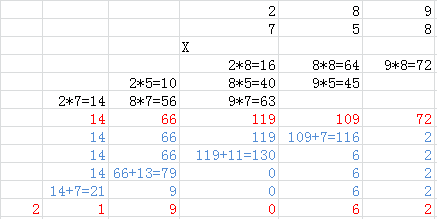
\includegraphics[width=0.8\linewidth]{0043.png}
\end{center}
\subsection{44}
\begin{CJK}{UTF8}{gbsn}
	
\end{CJK}
\subsection{45}
\begin{CJK}{UTF8}{gbsn}
	
\end{CJK}
\subsection{46}
\begin{CJK}{UTF8}{gbsn}
	
\end{CJK}
\subsection{47}
\begin{CJK}{UTF8}{gbsn}
	
\end{CJK}
\subsection{48}
\begin{CJK}{UTF8}{gbsn}
	
\end{CJK}
\subsection{49}

\section{SOLUTION}
\subsection{40}
\subsection{41}
\subsection{42}
\begin{enumerate}
\item
\begin{lstlisting}
int trap( int A[], int n ) {
	int res = 0, left = 0, right = 0, level = 0;
	for ( int i = 1; i < n - 1; ++i ) {
		if ( A[i] >= A[i - 1] || A[i] > A[i + 1] ) continue;
		for ( left = i - 1; left > 0; --left ) {
			if ( A[left] >= A[left - 1] ) break;
		}
		right = i + 1;
		for ( int j = i + 1; j < n; ++j ) {
			if ( A[j] >= A[right] ) {
				right = j;
				if ( A[right] >= A[left] ) break;
			}
		}
		level = min( A[left], A[right] );
		for ( int j = left + 1; j < right; ++j ) {
			if ( level - A[j] > 0 ) res += (level - A[j]);
		}
		i = right;
	}
	return res;
}
\end{lstlisting}
\item
\begin{lstlisting}
int trap( int A[], int n ) {
	int res = 0, mx = 0;
	vector<int> dp( n, 0 );
	for ( int i = 0; i < n; ++i ) {
		dp[i] = mx;
		mx = max( mx, A[i] );
	}
	mx = 0;
	for ( int i = n - 1; i >= 0; --i ) {
		dp[i] = min( dp[i], mx );
		mx = max( mx, A[i] );
		if ( dp[i] - A[i] > 0 ) res += (dp[i] - A[i]);
	}
	return res;
}
\end{lstlisting}
\item
\begin{lstlisting}
int trap( int A[], int n ) {
	int res = 0, left = 0, right = n - 1;
	while ( left < right ) {
		int mn = min( A[left], A[right] );
		if ( A[left] == mn ) {
			++left;
			while ( left < right && A[left] < mn ) {
				res += (mn - A[left]);
				++left;
			}
		}
		else {
			--right;
			while ( left < right && A[right] < mn ) {
				res += (mn - A[right]);
				--right;
			}
		}
	}
	return res;
}
\end{lstlisting}
\end{enumerate}

\subsection{43}
\begin{lstlisting}
string multiply( string num1, string num2 ) {
	string res;
	int n1 = num1.size(), n2 = num2.size();
	int k = n1 + n2 - 2, carry = 0;
	vector<int> v( n1 + n2, 0 );
	for ( int i = 0; i < n1; ++i ) {
		for ( int j = 0; j < n2; ++j ) {
			//add without carry
			v[k - i - j] += (num1[i] - '0') * (num2[j] - '0');
		}
	}
	for ( int i = 0; i < n1 + n2; ++i ) {
		v[i] += carry;
		carry = v[i] / 10;
		v[i] %= 10;
	}
	int i = n1 + n2 - 1;
	while ( v[i] == 0 ) --i; //remove "0" as prefix
	if ( i < 0 ) return "0"; //remove zero
	while ( i >= 0 ) res.push_back( v[i--] + '0' );
	return res;
}
\end{lstlisting}
\subsection{44}
\subsection{45}
\subsection{46}
\subsection{47}
\subsection{48}
\subsection{49}
\end{document}